\documentclass[a4paper]{article}
\usepackage{amsmath,multicol,graphicx}
\renewcommand{\d}{\ensuremath{\mathrm{d}}}
\newcommand{\der}[2]{\ensuremath{\frac{\d \, #1}{\d \, #2}}}
\newcommand{\pder}[2]{\ensuremath{\frac{\partial \, #1}{\partial \, #2}}}
\newcommand{\CC}{C\nolinebreak\hspace{-.05em}\raisebox{.4ex}{\tiny\bf +}\nolinebreak\hspace{-.10em}\raisebox{.4ex}{\tiny\bf +}}
\newcommand{\textdegree}{\ensuremath{^{\circ}}}

\title{DMFC system modelling}
\author{Federico Zenith}

\begin{document}
\maketitle

\begin{abstract}
This document describes the classes and formulas used in the DMFC system
modelling.
Remark that all models assume environmental pressure in all parts, i.e.
$p = 101325\, \mathrm{Pa}$.
\end{abstract}

\section*{Nomenclature}
\setlength{\columnsep}{1pc}
\setlength\columnseprule{.4pt}
\begin{multicols}{2}
\begin{tabbing}
\hspace{0.75cm} \= \hspace*{3.5cm} \= \kill
$A$ \> Area \> [m\textsuperscript{2}]\\
$c_p$ \> Specific heat capacity \> [J/mol\,K]\\
$C_p$ \> Heat capacity \> [J/K]\\
$h$ \> Molar enthalpy \> [J/mol]\\
$\Delta h_f^0$ \> Formation enthalpy \> [J/mol]\\
$\dot H$ \> Enthalpy flow \> [W]\\
$k_h$ \> Heat transfer coeff. \> [W/K] \\
$l$ \> Level \> [m] \\
$M$ \> Molar mass \> [kg/mol]\\
$n$ \> Number of moles \> [mol]\\
$\dot n$ \> Molar flow \> [mol/s]\\
$p$ \> Pressure \> [Pa]\\
$p^0$ \> Vapour pressure \> [Pa]\\
$\dot Q$ \> Heat flow \> [W]\\
$T$ \> Temperature \> [K]\\
$U$ \> Internal energy \> [J]\\
$x$ \> Liquid molar fraction \> [-] \\
$y$ \> Gaseous molar fraction \> [-] \\
$z$ \> Overall molar fraction \> [-] \\
$V$ \> Volume \> [m\textsuperscript{3}]\\
$\rho$ \> Density \> [kg/m\textsuperscript{3}]\\
\\\textbf{Subscripts}\\
$g$ \> Gas phase\\
$l$ \> Liquid phase\\
ref \> Reference state\\
env \> Environment\\
\textbf{Capitalisation}\\
$A$ \> Extensive unit \> e.g. J\\
$a$ \> Intensive molar unit \> e.g. J/mol\\
$\hat a$ \> Intensive mass unit \> e.g. J/kg\\
$\tilde a$ \> Intensive volume unit \> e.g. J/m\textsuperscript{3}
\end{tabbing}
\end{multicols}


\section{Thermodynamics Library}
The thermodynamics library provides a number of properties necessary for the
simulation environment. The library is placed in the Modelica package
\texttt{Thermo}, and comprises constants and functions for:

\begin{itemize}
\item molar mass $M$,
\item molar enthalpy $h(T)$,
\item molar specific heat capacity $c_p(T)$,
\item heat of formation at standard conditions $\Delta h_f^0$,
\item vapour pressure (only water and methanol) $p^0(T)$,
\item density $\rho(T)$.
\end{itemize}

Where not otherwise specified, the functions are provided for five components,
identified by the numbers:

\begin{enumerate}
\item methanol,
\item water,
\item oxygen,
\item carbon dioxide,
\item nitrogen.
\end{enumerate}

Some functions are also applicable for different phases; it is assumed that only
methanol and water can be in liquid phase. Phases are identified as follows:

\begin{enumerate}
\item gaseous,
\item liquid.
\end{enumerate}

The code uses \emph{pseudo-enumerations}, that is there are a number of integer
variables named after the components (Methanol, Water, . . . ) with the appro-
priate name. These must be imported in functions using them, as in import
Thermo.Nitrogen.


\section{Tanks and Flows}
The bulk of the model is done by means of \emph{continuously stirred tanks}.
These are very generic tanks with uniform intensive properties (temperature,
composition, pressure and so on) that can actually be used to represent pipes
(e.g. a large number of small tanks in series approximate a plug flow).

Tanks are connected to each other by means of \texttt{FlowConnector}s.


\subsection{The \texttt{CheckPoint} Connector Class}
A \texttt{CheckPoint} represents what passes through a certain area on the
control volume, corresponding to inlets and outlets. It does not have an own
volume.

\begin{figure}[h]
\centering
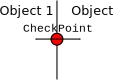
\includegraphics[width=0.4\textwidth]{pics/checkpoint}
\end{figure}

This connector class contains:

\begin{itemize}
\item the total molar flow $\dot n$ (mol/s);
\item five molar fractions of the passing flow, $z_i$;
\item the total enthalpy flow $\dot H$ (W).
\item the molar fractions of the tank and phase it belongs to,
$z^\text{local}_i$;
\item the specific enthalpy of the tank it belongs to, $h^\text{local}$;
\end{itemize}

For flows, the general sign rule is that \emph{the system is the subject}:
positive is entering, negative is exiting.

The reasons for using enthalpy flow instead of the more usual temperature are:

\begin{itemize}
\item flows could be in two phases (and we would then have to describe these);
\item flows could be not in equilibrium;
\item in any case, when mixing flows at different temperatures, we would end up
calculating the enthalpy anyway.
\end{itemize}

The enthalpy flow is given according to the assumption that our
\textbf{reference state} is:

\begin{itemize}
\item at 298.15\,K;
\item with methanol and water completely in liquid phase;
\item with oxygen, nitrogen and carbon dioxide in gas phase.
\end{itemize}

Note that sanity checks ($\sum_i z_i = 1$, $z_i \in [0,1] ~ \forall i$)
\emph{cannot} be implemented in \texttt{CheckPoint}, because connector classes
are not allowed to have any kind of equations, there included
\texttt{assert}ions. The checks will be implemented in \texttt{StirredTank}.

Note also that molar and enthalpy flows are not implemented with the Modelica
\texttt{flow} keyword. The connection is instead done ``manually'' in class
\texttt{FlowConnector} because of the necessity of a separate class to decide
which $\mathbf{z}^\text{local}$ and $h^\text{local}$ to use for $\mathbf{z}$ and
$\dot H$.


\subsection{The \texttt{FlowConnector} Pseudo-Connector}
\texttt{FlowConnector}s are actually not standard Modelica connectors, because
they contain equations. They are \emph{discriminating models}, that are used to
determine the composition and enthalpy of a flow.

When connecting two tanks, it is not possible to determine the composition and
enthalpy content of a flow from either tank: to do that, it is necessary to have
information about \emph{both} tanks (their composition and their specific
enthalpy. These are specified when setting $\mathbf{z}^\text{local}$ and
$h^\text{local}$ in \texttt{CheckPoints} (either to overall values or to those
of a specific phase).

The \texttt{FlowConnector} class takes the value of flow, makes sure that $F_1
+F_2=0$, and determines which local values of specific enthalpy and
composition will be used between its first and second port.


\subsection{The \texttt{StirredTank} Abstract Class}
This class is \emph{abstract} in the sense it is not supposed to be used
directly, but only through inheritance to other classes. This class lacks
important details, such as a defined shape, but specifies the generic behaviour
common to all tanks.

\begin{figure}[h]
\centering
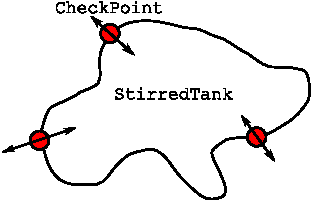
\includegraphics[width=0.4\textwidth]{pics/stirredtank}
\end{figure}

The \texttt{StirredTank} class handles:
\begin{itemize}
\item mass balances;
\item heat balance;
\item liquid-vapour equilibria;
\item sanity checks.
\end{itemize}

The class seeks environment temperature and pressure $T_\text{env}$ and
$p_\text{env}$ in the containing classes (see Modelica reference books for
scoping rules and the \texttt{inner} and \texttt{outer} keywords). This means
that, when the total model is built, these variables should be defined in one
place only, and all instances of \texttt{StirredTank} will use them.

Its parameters are the heat capacity $C_p$ of the tank itself (glass, lid,
etc.), the heat transfer coefficient $k_h$, the number of connected flows $m$
(note that at this point it is left unspecified), its volume $V$ and a string
with its name.

Its variables are the temperature $T$, initialised at $T_\text{env}$, five
amounts of moles $\mathbf{n}$, one for each component, the heat exchanged with
the environment $\dot Q$, and the \texttt{CheckPoint}s representing the
connected flows (whose number, we repeat, is still left unspecified).

For the two phases, there are variables $n_g$ and $n_l$ (total moles in gas and
liquid phase), the volumes $V_g$ and $V_l$ taken up by each phase, and the
molar-fraction vectors $\mathbf{y}$ and $\mathbf{x}$.

\subsubsection{Equations}
The \textbf{mass balance} is straightforward:

\begin{equation}
\der{\mathbf{n}}{t} = \sum_{j \in [1, m]} \mathbf{z}_j\,F_j
\end{equation}

The derivative of the moles of each component is simply the sum of all inlets,
some of which may be negative (and therefore an outlet). We are assuming here
that we have no reaction.

The \textbf{energy balance} is more intricate. First, the differential equation
for the internal energy contained by the tank:

\begin{equation}
\label{firstlaw}
\der{U}{t} = \dot Q + \sum_{j \in [1, m]} \dot H_j
\end{equation}

Heat exchange with the environment is modelled simply as:

\begin{equation}
\dot Q = k_h ( T_\text{env} - T )
\end{equation}

We can also express the internal energy $U$ as a function of temperature and
composition:

\begin{multline}
\label{Ugeneral}
U(T, n_i, n_{g,i}) = C_p \, ( T - T_\text{ref} ) +
\sum_j \left (\Delta h _{g,j}^f - \Delta h _{l,j}^f \right) \, n_{g,j} \\
+ \sum_{i,j} [ h_{i,j}(T) - h_{i,j}(T_\text{ref})] \, n_{i,j}
\end{multline}


Where the first term on the right-hand side indicates the heat content of the
tank itself; in the second term we usually consider only water
and methanol (the only species that can evaporate from liquid state), whereas
in the third term we consider all species, counting separately the same species
in different phases.

Equation \ref{Ugeneral} states that the internal energy for a certain
temperature and composition is the evaporation enthalpy at the standard
temperature and the sensible heat to bring the components from standard to
actual temperature. It could have been done the other way around, but this is
simpler.

The total derivative of internal energy is by definition:
\begin{equation}
\label{totalDerU}
\der{U}{t} = \pder{U}{T}\,\der{T}{t} + \sum_i \pder{U}{n_i}\,\der{n_i}{t} +
\sum_j \pder{U}{n_{g,j}}\,\der{n_{g,j}}{t}
\end{equation}

The partial derivative terms are calculated from equation \ref{Ugeneral}:

\begin{align}
\pder{U}{T} & = C_p + \sum_i c_{p,i} n_i\\
\pder{U}{n_i} & = h_i(T) - h_i(T_\text{ref})\\
\pder{U}{n_{g,j}} & = \Delta h _{g,j}^f - \Delta h _{l,j}^f
\end{align}

Putting this together with equation \ref{firstlaw}, we obtain:

\begin{equation}
\boxed{ \begin{aligned}
k_h ( T_\text{env} - T ) + \sum_{j \in [1, m]} \dot n_{ij} = &
\overbrace{\left ( C_p + \sum_i c_{p,i} n_i \right) \der{T}{t} }
^\text{Sensible heat} +\\
& \overbrace{\sum_j [ \Delta h _{g,j}^f - \Delta h _{l,j}^f ] \der{n_{g,j}}{t}}
^\text{Latent heat} +\\
& \overbrace{ \sum_i [ h_i(T) - h_i(T_\text{ref}) ] \der{n_i}{t} }
^\text{New mass}
\end{aligned} }
\end{equation}


The \textbf{liquid-vapour equilibrium} requires us to define the molar fractions
of all components in liquid and gaseous phase, respectively $x_i$ and $y_i$;
these must satisfy:

\begin{align}
\sum_i x_i &= 1\\
\sum_i y_i &= 1
\end{align}

The equilibrium equations are the Raoult law for water and methanol, and that
there is no gaseous species in liquid phase:

\begin{align}
p_\text{env} \, y_i &= p^0_i(T) \, x_i & \forall \, i \in \lbrace \mathrm{H_2O, CH_3OH} \rbrace\\
x_i &= 0 & \forall \, i \in \lbrace \mathrm{O_2, CO_2, N_2} \rbrace
\end{align}

The compositions are related to the total moles in the tank:

\begin{equation}
\mathbf{n} = n_l\,\mathbf{x} + n_g\,\mathbf{y}
\end{equation}

In turn, the moles in liquid and gaseous phase,  $n_l$ and $n_g$ respectively,
are bound to the respective volumes:

\begin{align}
V_l &= \sum_i \frac{n_l \, x_i \, M_i}{\rho_i(T)}\\
V_g &= \sum_i \frac{n_g \, y_i \, M_i}{\rho_i(T)}
\end{align}

In these equations it has been assumed that there is no mixing volume, and the
density of gaseous components is calculated with the ideal-gas law.

Finally, the gas and liquid volumes are bound to the total tank volume $V$,
which is a parameter of the tank model (whereas $V_l$ and $V_g$ are variables).

\begin{equation}
V = V_g + V_l
\end{equation}

Equilibrium is an algebraic (as opposed to differential) equation set. We have
defined 15 equations and introduced 14 variables.

\subsubsection{Sanity checks}
The tank model will use the \texttt{assert} function to make sure that certain
consistency conditions are always true: if these were not, it would be an
indicator of errors in the model, and the model should be stopped at that exact
moment to help pinpoint the issue.

The following conditions should always be true:
\begin{align}
n_i & \geq 0 & \forall \, i\\
x_i & \in [0,1] & \forall \, i\\
y_i & \in [0,1] & \forall \, i\\
n_g & \geq 0\\
n_l & \geq 0\\
V_g & \geq 0\\
V_l & \geq 0
\end{align}

In practice, to account for numerical noise, these comparisons are usually
with $-\epsilon$ instead of 0.

\subsubsection{Initialisation}
Initialisation of the tank simulation is not trivial, because it is possible to
specify a set of starting values for the differential variables ($\mathbf{n}$
and $T$) that does not have a total volume of $V$; trivially, $\mathbf{n} =
\mathbf{0}$ is inconsistent with our assumption of $p$ being always 101325\,Pa.

Therefore, we must be able to modify at least one $n_i$. None of the $n_i$ have
their \texttt{fixed} attribute set to \texttt{true}, so the initialisation is
free to choose any consistent start state.

If children classes want to implement particular policies (such as ``change the
air content'' or ``fill with water''), they will have to \texttt{redeclare} the
variable with the appropriate, or to define an \texttt{initial equation}.

\subsection{The \texttt{VerticalCylindricalTank} Class}
This class inherits from \texttt{StirredTank}, and gives it a defined shape.
It adds a variable level and a parameter $A$ for the cross-sectional area.

Since the liquid-gas interface is parallel to the cross section, the level is
simply:

\begin{equation}
l = \frac{V_l}{A}
\end{equation}

\subsection{The \texttt{HorizontalCylindricalTank} Class}
This class inherits too from \texttt{StirredTank} and gives it a cylindrical
shape, but its expression for the level is not as simple as for
\texttt{VerticalCylindricalTank}.

\begin{figure}[h]
\centering
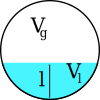
\includegraphics[width=0.3\textwidth]{pics/crosssection}
\end{figure}

Having defined a unity circle by the parametric equation $x^2+y^2=1$, we can
find the part of its area enclosed in the interval $[-1,z]$ with $z \in [-1,1]$
as follows:

\begin{equation}
A(z) = \int_{-1}^z 2 \, \sqrt{1-x^2} \, \d x
\end{equation}

Obviously, $A(1) = \pi$. We can make this relevant to our case by changing
variables as:

\begin{align}
\frac{A}{\pi} &= \frac{V_l}{V}\\
z &= 2\,\frac{l}{d}-1
\end{align}

where $d$ is the internal diameter of the cylinder (and the maximum level $l$).
The integral expression becomes:

\begin{equation}
\frac{V_l}{V} = \frac{2}{\pi} \int_{-1}^{2\frac{l}{d}-1} \sqrt{1-z^2} \, \d z
\end{equation}

Whose solution is:

\begin{equation}
\pi \, \frac{V_l}{V} = 2 \left(2\,\frac{l}{d} -1 \right)\sqrt{\frac{l}{d}-
\frac{l^2}{d^2}} + \arcsin\left(2\,\frac{l}{d} -1 \right) + \frac{\pi}{2}
\end{equation}

The plot of $l$ versus $V_l$ is however not very far from linear, deviating from
a linear relationship by at most 6\,\% of the total height.


\subsection{The \texttt{PipeSegment} Class}
A \texttt{PipeSegment} is a specialised \texttt{StirredTank} with two
\texttt{CheckPoint}s. For each of the class' \texttt{CheckPoint}s, the values
of $\mathbf{z}^\text{local}$ and $h^\text{local}$ are set as the average molar
fractions $\mathbf{z}$ and enthalpy $h_\text{tot}$ of the tank.


\subsection{The \texttt{Pipe} Class}
The \texttt{Pipe} class is composed of a generic number $n$ of
\texttt{PipeSegment}s, which are connected in series with hidden
(\texttt{protected}) \texttt{FlowConnectors}. The pipe segments are a
\texttt{replaceable} type, so that the \texttt{Pipe} class can be used later on
with different types of segments.


\subsection{The \texttt{HeatExchangerPipeSegment} Class}
This is a child class of \texttt{PipeSegment}, with one more \texttt{CheckPoint}
to pass a heat flow through. This \texttt{CheckPoint}'s $F$ and $\mathbf{z}$ are
set to zero.


\subsection{The \texttt{HeatExchangerPipe} Class}
This is a child class of \texttt{Pipe}, where the segments are now of type
\texttt{HeatExchangerPipeSegments}. It is otherwise identical to its parent
class.


\subsection{The \texttt{HeatExchanger} Class}
Heat exchangers are modelled with two \texttt{HeatExchangerPipe}s representing
the two sides and a number of parameters, namely:

\begin{itemize}
\item area $A$,
\item coefficient of heat transfer $U$,
\item number of discretisation steps,
\item total volumes of the two sides $V_1$ and $V_2$.
\end{itemize}

The two \texttt{HeatExchangerPipe}s are instantiated with an equal number of
segments, defined by the exchanger's number of steps. For each step, the
enthalpy flow of the extra \texttt{CheckPoint} introduced in
\texttt{HeatExchangerPipeSegment} is used to transfer heat between the sides.
For each step, it is set that $H_1+H_2=0$ and that the flow of heat is:

\begin{equation}
H_1 = \frac{A}{\text{steps}}\,U\,(T_2-T_1)
\end{equation}

The heat exchanger includes another variable, $Q$, which is the sum of all the
heat transferred from the first to the second side.

Since this is a dynamic model, it is not possible to use steady-state techniques
such as the LMTD: indeed, during a transient it is possible that the temperature
profiles along the exchanger will cross.


\subsection{The \texttt{FlowController} Class}
A \texttt{FlowController} is a class that containts two \texttt{CheckPoint}s,
and allows to set the mass flow rate through the unit.


\subsection{The \texttt{GasFlowController} Class}
This is a class derived from \texttt{FlowController}; it adds the possibility
of setting a volumetric flow. It is assumed that \emph{all components are in
gas phase}.

In order to set the volumetric flow as a function of mass flow, it is necessary
to set a reference temperature, which can be done with the $T$ parameter; this
defaults to 273.15\,K, the so-called ``standard''. The ``norm'', instead, is at
70\,\textdegree F, or $\approx$21\,\textdegree C. Other standards use
25\,\textdegree C.


\subsection{The \texttt{Pump} class}
This is another derived class of \texttt{FlowController}, and just like
\texttt{GasFlowController} it gives the possibility to set the volumetric flow;
only, this is done \emph{assuming all flow is liquid} and that all flow is
either water or methanol.


\end{document}
